% POLAR 15.4 
\ifnum \Version=1
    \part Using polar coordinates, the average value of $f(x,y) = 18x^2y$ over the region in the region in the first quadrant bounded by $x^2+y^2=9$ is $\displaystyle  \int_a^b \int_c^d g(r,\theta) \, dr \, d\theta$,  where $a=\framebox{\strut\hspace{1cm}}$, $b=\framebox{\strut\hspace{1cm}}$, $c=\framebox{\strut\hspace{2cm}}$, $d=\framebox{\strut\hspace{2cm}}$, and $g(r,\theta) = \framebox{\strut\hspace{2cm}}$.

    \ifnum \Solutions=1 
    {\color{DarkBlue} 
    The average value of a function $f(x,y)$ over a region $R$ is given by 
    \begin{align}
        \text{Average value of }f\text{ over region }R 
        &= \frac{1}{\text{area of region }R}\iint_R f \, dA \\
        &= \iint_R \frac{f(x,y)}{\text{area of region }R} \, dA
    \end{align}
    We want to convert this expression to polar so that we can write
        \begin{align}
        \text{Average value of }f\text{ over region }R 
        &= \iint_R \frac{f(x,y)}{\text{area of region }R} \, dA 
        = \int_a^b \int_c^d g(r,\theta) \, dr \, d\theta
    \end{align}
    In polar, we use $$dA = r \, dr \, d\theta$$ So to obtain $g$ in terms of $r$ and $\theta$, we can use
    \begin{align}
         g \, dr \, d\theta &= \frac{f(x,y)}{\text{area of region }R}  \, dA \\
         &= \frac{f(x(r,\theta),y(r,\theta))}{\text{area of region }R} \ r \, dr \, d\theta  \\ 
        g &= \frac{f(r,\theta)}{\text{area of region }R} \ r
    \end{align}
    So we need to express $f$ in terms of $r$ and $\theta$, and we need the area of the region. To express $f$ in terms of $r$ and $\theta$ we use $x=r\cos\theta$ and $y=r\sin\theta$. 
    \begin{align}
        f(x,y) = f(x(r,\theta),y(r,\theta)) = 18x^2y = 18r^3\cos^2\theta \sin\theta
    \end{align}
    To determine the area of $R$, it can help to sketch the region, as shown in the diagram below. 
    \begin{center}     
    \begin{tikzpicture}[scale=0.75]
        \begin{axis}[
        axis lines = middle, very thick,
        xlabel = {$x$},
        ylabel = {$y$},
        xmin=-1, xmax=4.75,
        ymin=-1, ymax=4.5,
        xtick={0,1,2,3},
        xticklabels={0,1,2,3},  
        ytick={0,1,2,3},
        yticklabels={0,1,2,3},    
        ]
        % Plot 1
        \addplot [name path = A,
        -,
        domain = 0:3, ultra thick,DarkBlue,
        samples = 100] {sqrt(9-x^2} 
        node [right=2pt] {};
        \node (l) at (3,3) {$x^2+y^2 = 9$};
        \node (l) at (1.25,1.25) {$R$};
        \addplot[ultra thick, samples=50, smooth,domain=0:3,DarkBlue] coordinates {(0,0)(0,3)};        
        \addplot [name path = B,
        -,
        domain = 0:3, ultra thick,DarkBlue,
        samples = 100] {0} 
        node [very near end, right=4pt] {}; 
        % Fill area between paths
        \addplot [black!30, opacity=0.2] fill between [of = A and B, soft clip={domain=0:3}];
        \end{axis}
    \end{tikzpicture}    
    \end{center}     
    The area of the region is a quarter of the area of a circle with radius $r=3$. 
    $$\text{area of region} = \frac{\pi r^2}{4} = \frac{9\pi}{4}$$
    The region is 
    $$R = \{(r,\theta) \in \mathbb R^2 \, | \, 0 \le r \le 3, \ 0 \le \theta \le \pi/2 \}$$
    Therefore, 
    \begin{align}
        a & = 0 \\
        b &= \pi/2 \\
        c &= 0 \\
        d &= 3 \\
        g &= \frac{f(x,y)}{\text{area of region}} r = \frac{18r^4\cos^2\theta \sin\theta}{9\pi/4} = \frac{8r^4\cos^2\theta \sin\theta}{\pi}
    \end{align}
    }
   \else

   \fi
\fi 




% 15.4
% FROM THOMAS, 15.4, #16
\ifnum \Version=2
    \part $\displaystyle \int_{\sqrt2}^{2}\int_{\sqrt{4-y^2}}^{y} x^2+y^2 \, dx \, dy = \int_a^b \int_c^d f(r,\theta) \, dr \, d\theta$ where $a=\framebox{\strut\hspace{0.8cm}}$, $b=\framebox{\strut\hspace{0.8cm}}$, $c=\framebox{\strut\hspace{0.8cm}}$, $d=\framebox{\strut\hspace{0.8cm}}$, and $f(r,\theta) = \framebox{\strut\hspace{2cm}}$.
    
    \ifnum \Solutions=1 
    {\color{DarkBlue}
    The region is bounded by the curves
    $$x = \sqrt{4-y^2}, \ x = y, \ y = \sqrt2, \ y = 2$$
    The region lies outside the circle $x^2+y^2=4$, and between the lines $y=x$ and $y=2$. The line $y=2$ in polar coordinates becomes
    \begin{align}
        y = 2 = r\sin\theta \quad \Rightarrow \quad r = 2 \csc\theta
    \end{align}
    Converting the integrand $x^2+y^2$ into polar we obtain 
    \begin{align}
        x^2+y^2 = r^2
    \end{align}
    After converting the above integral to polar we obtain 
    \begin{align}
        \int_{\sqrt2}^{2}\int_{\sqrt{4-y^2}}^{y} x^2+y^2 \, dx \, dy =  \int_{\pi/4}^{\pi/2}\int_2^{2\csc\theta} (r^2) r \, dr \, d\theta 
    \end{align} 
    Thus,
    \begin{align}
        a &= \pi/4 \\
        b &= \pi/2 \\
        c&= 2 \\
        d&=2 \csc\theta \\
        f(r,\theta) &= r^3
    \end{align}
    }
   \else

   \fi
    
\fi





% OOOPS! NO VERSION 3!!! 






% 15.4
% BASED ON  THOMAS, 15.4, #13
% TRIANGULAR REGION FIRST QUADRANT
\ifnum \Version=4
    \part $\displaystyle \int_{0}^{6}\int_{0}^{y} y \, dx \, dy = \int_a^b \int_c^d f(r,\theta) \, dr \, d\theta$,  where $a=\framebox{\strut\hspace{1.42cm}}$, $b=\framebox{\strut\hspace{1.42cm}}$, $c=\framebox{\strut\hspace{2cm}}$, $d=\framebox{\strut\hspace{2cm}}$, and $f(r,\theta) = \framebox{\strut\hspace{2cm}}$.
    
    \ifnum \Solutions=1 
    {\color{DarkBlue}
    The region is bounded by
    $$0\le y \le 6, \quad 0 \le x \le y$$
    It can help to sketch the region, as shown in the diagram below. 
       \begin{center}     
        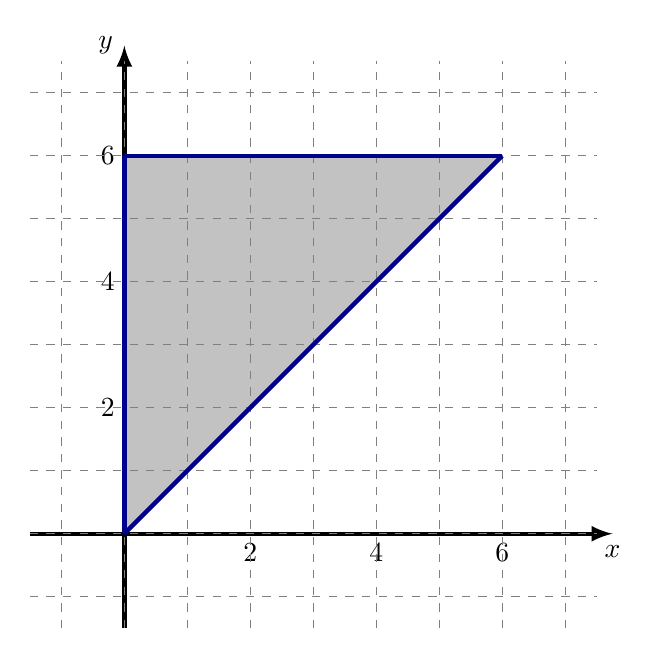
\begin{tikzpicture}[scale=0.8]
        \draw[fill=gray!80!black, opacity=0.4] (0,0) -- (0,6) -- (6,6);        
        \draw[ultra thick,->,>=latex] (-1.5,0)--(7.75,0) node[below] {$x$};
        \draw[ultra thick,->,>=latex] (0,-1.5)--(0,7.75) node[left] {$y$};       
        \draw (2,0) node[below] {$2$};          
        \draw (4,0) node[below] {$4$};          
        \draw (6,0) node[below] {$6$};          
        \draw (0,2) node[left] {$2$};        
        \draw (0,4) node[left] {$4$};
        \draw (0,6) node[left] {$6$};
        \draw[help lines,gray,thin,dashed] (-1.5, -1.5) grid (7.5, 7.5);
        \draw[domain=0:6,ultra thick,DarkBlue,samples=200] plot ({\x},{\x});
        \draw[domain=0:6,ultra thick,DarkBlue,samples=200] plot ({\x},{6});
        \draw[ultra thick,-,DarkBlue,>=latex] (0,0)--(0,6);
    \end{tikzpicture}
    \end{center}     
    The line $y=6$ in polar becomes
    \begin{align}
        y=6 \quad \Rightarrow \quad r\sin\theta = 6 \quad \Rightarrow \quad r = 6 \csc \theta
    \end{align}
    Converting $y \, dx \, dy$ into polar, 
    \begin{align}
        y \, dx \, dy = (r\sin\theta ) r \, dr \, d\theta =  r^2\sin\theta \, dr \, d\theta
    \end{align}
    Converting the integral from Cartesian to polar we obtain 
    \begin{align}
        \int_{\pi/4}^{\pi/2} \int_{0}^{6\csc\theta} r^2\sin\theta \, dr \, d\theta 
    \end{align} 
    Thus,
    \begin{align}
        a &= \pi/4 \\
        b &= \pi/2 \\
        c&= 0 \\
        d&= 6\csc\theta \\
        f(x,y) &= r^2\sin\theta
    \end{align}
    }
   \else

   \fi
    
\fi












% 15.4
% QUARTER CIRCLE WITH WEIRD RADIUS
\ifnum \Version=5
    \part $\displaystyle \int_0^{2}\int_{x}^{\sqrt{8-x^2}} \, dy \, dx = \int_a^b \int_c^d r\, dr \, d\theta$ where $a=\framebox{\strut\hspace{0.8cm}}$, $b=\framebox{\strut\hspace{0.8cm}}$, $c=\framebox{\strut\hspace{0.8cm}}$, $d=\framebox{\strut\hspace{0.8cm}}$.
    
    \ifnum \Solutions=1 
    {\color{DarkBlue}
    The region is the quarter circle bounded by the curves
    $$x = 0, \ x = 2, \ y = x, \ x^2+y^2 = 8$$
    The line $y=x$ intersects $x^2+y^2=8$ when
    \begin{align}
        (y)^2 + y^2 &= 8 \\
        2y^2 &= 8 \\
        y &= \pm 2
    \end{align}
    We only need the positive value. The curves intersect at $(2,2)$. After converting these curves to polar we obtain 
    \begin{align}
        \int_0^{2}\int_{x}^{\sqrt{8-x^2}} \, dy \, dx 
        \ =  \int_{\pi/4}^{\pi/2}\int_0^{\sqrt{8}} r \, dr \, d\theta 
    \end{align} 
    Thus,
    \begin{align}
        a &= \pi/4 \\
        b &= \pi/2 \\
        c&= 0 \\
        d&=\sqrt8
    \end{align}
    It is ok to use $d=2\sqrt2$. 
    }
   \else

   \fi
    
\fi





% 15.4
% BASED ON  THOMAS, 15.4, #25
% TRIANGULAR REGION IN FIRST AND 2ND QUADS
\ifnum \Version=6
    \part $\displaystyle \int_{\pi/4}^{3\pi/4}\int_{0}^{4\csc\theta} r^2\sin\theta \, dr \, d\theta = \int_a^b \int_c^d f(x,y) \, dx \, dy$,  where $a=\framebox{\strut\hspace{1.42cm}}$, $b=\framebox{\strut\hspace{1.42cm}}$, $c=\framebox{\strut\hspace{2.5cm}}$, $d=\framebox{\strut\hspace{2.5cm}}$, and $f(x,y) = \framebox{\strut\hspace{2.5cm}}$.
    
    \ifnum \Solutions=1 
    {\color{DarkBlue}
    The region is the triangular area bounded by the curves
    $$r = 4\csc\theta, \ \theta  =  \pi/4 , \ \theta = 3\pi/4$$
    
    The line $r=4\csc\theta$ in rectangular coordinates becomes
    \begin{align}
        r=4\csc\theta \quad \Rightarrow \quad r\sin\theta = 4 \quad \Rightarrow \quad y = 4
    \end{align}
    The lines $\theta  = \pi/4 , \theta = 3\pi/4$ become $y=x$ and $y=-x$.  It can help to sketch the region, as shown in the diagram below. 
       \begin{center}     
        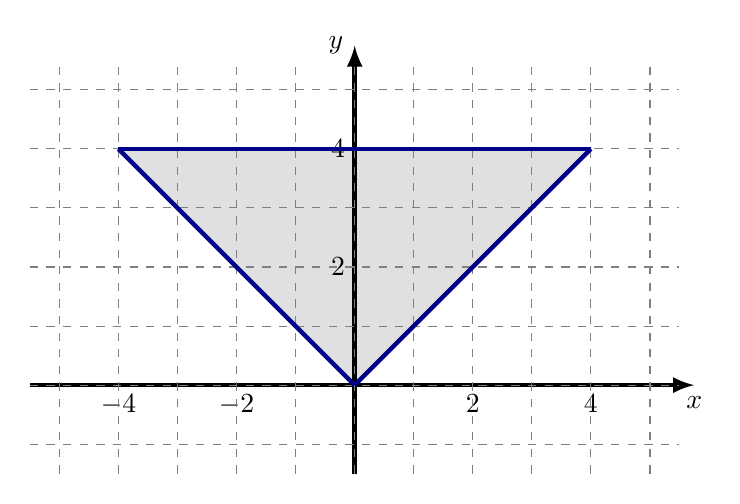
\begin{tikzpicture}[scale=0.75]
        \draw[fill=gray!80!black, opacity=0.2] (0,0) -- (4,4) -- (-4,4);        
        \draw[ultra thick,->,>=latex] (-5.5,0)--(5.75,0) node[below] {$x$};
        \draw[ultra thick,->,>=latex] (0,-1.5)--(0,5.75) node[left] {$y$};       
        \draw (-2,0) node[below] {$-2$};          
        \draw (-4,0) node[below] {$-4$};  
        \draw (2,0) node[below] {$2$};          
        \draw (4,0) node[below] {$4$};          
        \draw (0,2) node[left] {$2$};
        \draw (0,4) node[left] {$4$};
        \draw[help lines,gray,thin,dashed] (-5.5, -1.5) grid (5.5, 5.5);
        \draw[domain=-4:0,ultra thick,DarkBlue,samples=200] plot ({\x},{-\x});
        \draw[domain=0:4,ultra thick,DarkBlue,samples=200] plot ({\x},{\x});
        \draw[ultra thick,-,DarkBlue,>=latex] (-4,4)--(4,4);
    \end{tikzpicture}
    \end{center}           
    Converting $r^2\sin\theta\, dr \, d\theta$ into Cartesian we obtain 
    \begin{align}
        r^2\sin\theta \, dr \, d\theta =  (r\sin\theta) r \, dr \, d\theta = y \, dx\,dy
    \end{align}    
    Using the integration order $dy \, dx$ would require two separate double integrals in Cartesian, and the question asked for only one double integral. And the question specified that we use $dx\,dy$. The region can be described as
    \begin{align}
        R = \{ (x,y) \in \mathbb R^2 \, | \, \ 0 \le y \le 4, \ -y\le x \le y \}
    \end{align}
    After converting the above integral from polar to Cartesian we obtain 
    \begin{align}
        \int_{\pi/4}^{3\pi/4}\int_{0}^{4\csc\theta} r^2\sin\theta \, dr \, d\theta = \int_{0}^4 \int_{-y}^y y \, dx \, dy
    \end{align} 
    Thus,
    \begin{align}
        a &= 0 \\
        b &= 4 \\
        c&= -y \\
        d&= y \\
        f(x,y) &= y
    \end{align}
    }
   \else

   \fi
    
\fi


% 15.4
% BASED ON  THOMAS, 15.4, #23
% USED AS AN EXAM QUESTION IN SPRING 2023
% QUARTER CRICLE IN 3RD QUAD
\ifnum \Version=7
    \part $\displaystyle \int_{\pi}^{3\pi/2}\int_{0}^{4} r^3\cos^2\theta \, dr \, d\theta = \int_a^b \int_c^d f(x,y) \, dy \, dx$,  where $a=\framebox{\strut\hspace{1.42cm}}$, $b=\framebox{\strut\hspace{1.42cm}}$, $c=\framebox{\strut\hspace{3cm}}$, $d=\framebox{\strut\hspace{3cm}}$, and $f(x,y) = \framebox{\strut\hspace{3cm}}$.
    
    \ifnum \Solutions=1 
    {\color{DarkBlue}
    The region is a quarter of a disc bounded by
    $$r = 4, \theta  = \pi , \ \theta = 3\pi/2$$
    The region is shown below. 
    \begin{center}  
    \begin{tikzpicture}[scale=0.75]
        \begin{axis}[
        axis lines = middle, very thick,
        xlabel = {$x$},
        ylabel = {$y$},
        xmin=-5, xmax=3.75,
        ymin=-5, ymax=3.75,
        xtick={-4,-2,0,2},
        xticklabels={-4,-2,0,2},
        ytick={-4,-2,0,2},
        yticklabels={-4,-2,0,2}        
        ]
        % Plot 1
        \addplot [name path = A,-,domain = -4:0, line width=0.8mm,DarkBlue,samples = 30] {-sqrt(16-x^2)} ;
        \addplot [name path = B,-,domain = -4:0, line width=0.8mm,DarkBlue,samples = 4]{0} node [very near end, right=4pt] {}; 
        % Vertical line
        \addplot[line width=0.8mm,samples=4, smooth,domain=0:6,DarkBlue, name path=three] coordinates {(0,0)(0,-4)};
        % Fill area between paths
        \addplot [black!30, opacity=0.2] fill between [of = A and B, soft clip={domain=-4:0}];
        \end{axis}
    \end{tikzpicture}    
    \end{center}    
    The curve $r=4$ in rectangular becomes
    \begin{align}
        r=4 \quad \Rightarrow \quad x^2 + y^2 = 4^2 \quad \Rightarrow \quad y = \pm \sqrt{16-x^2} 
    \end{align}
    Converting $r^3\cos^2\theta\, dr \, d\theta$ into Cartesian, 
    \begin{align}
        r^3\cos^2\theta \, dr \, d\theta =  x^2 \, dy\,dx
    \end{align}
    After converting the above integral from polar to Cartesian we obtain 
    \begin{align}
        \int_{\pi}^{3\pi/2}\int_{0}^{4} r^3\cos^2\theta \, dr \, d\theta 
        = \int_{-4}^0 \int_{-\sqrt{16-x^2} }^0 x^2 \, dy \, dx
    \end{align} 
    Thus,
    \begin{align}
        a &= -4 \\
        b &= 0 \\
        c&= -\sqrt{16-x^2} \\
        d&= 0 \\
        f(x,y) &= x^2
    \end{align}
    }
   \else

   \fi
    
\fi




% POLAR 
% 15.4
% TRIANGULAR REGION 2ND QUADRANT
\ifnum \Version=8
    \part $\displaystyle \int_{0}^{6}\int_{-y}^{0} x \, dx \, dy = \int_a^b \int_c^d f(r,\theta) \, dr \, d\theta$,  where $a=\framebox{\strut\hspace{1.42cm}}$, $b=\framebox{\strut\hspace{1.42cm}}$, $c=\framebox{\strut\hspace{2cm}}$, $d=\framebox{\strut\hspace{2cm}}$, and $f(r,\theta) = \framebox{\strut\hspace{2cm}}$.
    
    \ifnum \Solutions=1 
    {\color{DarkBlue}
    The region is bounded by
    $$0\le y \le 6, \quad -y \le x \le 0$$

    It can help to sketch the region, as shown in the diagram below. 
       \begin{center}     
        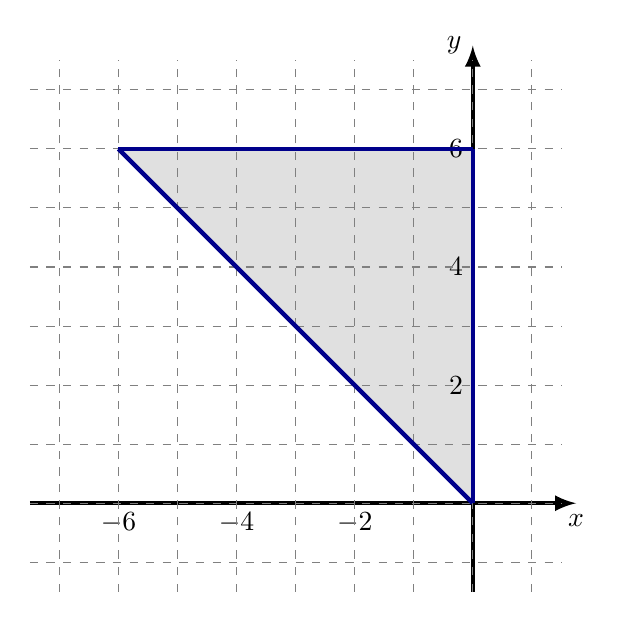
\begin{tikzpicture}[scale=0.75]
        \draw[fill=gray!80!black, opacity=0.2] (0,0) -- (0,6) -- (-6,6);        
        \draw[ultra thick,->,>=latex] (-7.5,0)--(1.75,0) node[below] {$x$};
        \draw[ultra thick,->,>=latex] (0,-1.5)--(0,7.75) node[left] {$y$};       
        \draw (-2,0) node[below] {$-2$};          
        \draw (-4,0) node[below] {$-4$};          
        \draw (-6,0) node[below] {$-6$};          
        \draw (0,2) node[left] {$2$};        
        \draw (0,4) node[left] {$4$};
        \draw (0,6) node[left] {$6$};
        \draw[help lines,gray,thin,dashed] (-7.5, -1.5) grid (1.5, 7.5);
        \draw[domain=-6:0,ultra thick,DarkBlue,samples=200] plot ({\x},{-\x});
        \draw[domain=-6:0,ultra thick,DarkBlue,samples=200] plot ({\x},{6});
        \draw[ultra thick,-,DarkBlue,>=latex] (0,0)--(0,6);
    \end{tikzpicture}
    \end{center}         
    The line $y=6$ in polar becomes
    \begin{align}
        y=6 \quad \Rightarrow \quad r\sin\theta = 6 \quad \Rightarrow \quad r = 6 \csc \theta
    \end{align}    
    Converting $x \, dx \, dy$ into polar, 
    \begin{align}
        x \, dx \, dy = (r\cos\theta ) r \, dr \, d\theta =  r^2\cos\theta \, dr \, d\theta
    \end{align}
    Converting the integral from Cartesian to polar we obtain 
    \begin{align}
        \int_{\pi/2}^{3\pi/4} \int_{0}^{6\csc\theta} r^2\cos\theta \, dr \, d\theta 
    \end{align} 
    Thus,
    \begin{align}
        a &= \pi/2 \\
        b &= 3\pi/4 \\
        c&= 0 \\
        d&= 6\csc\theta \\
        f(x,y) &= r^2\cos\theta
    \end{align}
    }
   \else

   \fi
    
\fi




% 15.4
% BASED ON  THOMAS, 15.4, #25
% TRIANGULAR REGION IN FIRST AND 4TH QUADS
\ifnum \Version=9
    \part $\displaystyle \int_{-\pi/4}^{\pi/4}\int_{0}^{3\sec\theta} r^3\sin^2\theta \, dr \, d\theta = \int_a^b \int_c^d f(x,y) \, dy \, dx$,  where $a=\framebox{\strut\hspace{1.42cm}}$, $b=\framebox{\strut\hspace{1.42cm}}$, $c=\framebox{\strut\hspace{2.5cm}}$, $d=\framebox{\strut\hspace{2.5cm}}$, and $f(x,y) = \framebox{\strut\hspace{2.5cm}}$.
    
    \ifnum \Solutions=1 
    {\color{DarkBlue}
    The region is the triangular area bounded by the curves
    $$r = 3\sec\theta, \ \theta  = - \pi/4 , \ \theta = \pi/4$$
    
    The line $r=3\sec\theta$ in rectangular coordinates becomes
    \begin{align}
        r=3\sec\theta \quad \Rightarrow \quad r\cos\theta = 3 \quad \Rightarrow \quad x = 3
    \end{align}
    The lines $\theta  = \pi/4 , \theta = -\pi/4$ become $y=x$ and $y=-x$.  Converting $r^3\sin^2\theta\, dr \, d\theta$ into Cartesian we obtain 
    \begin{align}
        r^3\sin^2\theta \, dr \, d\theta =  (r^2\sin^2\theta) r \, dr \, d\theta = y^2 \, dy\,dx
    \end{align}
    It can help to sketch the region, as shown in the diagram below. 
       \begin{center}     
        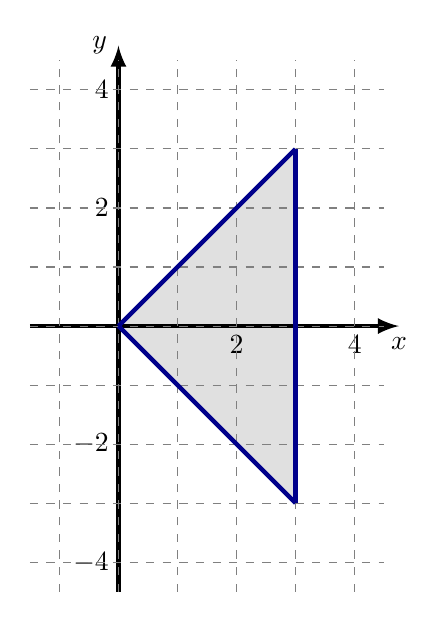
\begin{tikzpicture}[scale=0.75]
        \draw[fill=gray!80!black, opacity=0.2] (0,0) -- (3,3) -- (3,-3);        
        \draw[ultra thick,->,>=latex] (-1.5,0)--(4.75,0) node[below] {$x$};
        \draw[ultra thick,->,>=latex] (0,-4.5)--(0,4.75) node[left] {$y$};       
        \draw (2,0) node[below] {$2$};          
        \draw (4,0) node[below] {$4$};          
        \draw (0,-4) node[left] {$-4$};        
        \draw (0,-2) node[left] {$-2$};
        \draw (0,2) node[left] {$2$};
        \draw (0,4) node[left] {$4$};
        \draw[help lines,gray,thin,dashed] (-1.5, -4.5) grid (4.5, 4.5);
        \draw[domain=0:3,ultra thick,DarkBlue,samples=200] plot ({\x},{-\x});
        \draw[domain=0:3,ultra thick,DarkBlue,samples=200] plot ({\x},{\x});
        \draw[ultra thick,-,DarkBlue,>=latex] (3,-3)--(3,3);
    \end{tikzpicture}
    \end{center}           
    Using $dx \, dy$ would require two separate double integrals in Cartesian, and the question asked for only one double integral. And the question specified that we use $dy\,dx$. The region can be described as
    \begin{align}
        R = \{ (x,y) \in \mathbb R^2 \, | \, 0\le x \le 3, -x \le y \le x\}
    \end{align}
    After converting the above integral from polar to Cartesian we obtain 
    \begin{align}
        \int_{-\pi/4}^{\pi/4}\int_{0}^{3\sec\theta} r^3\sin^2\theta \, dr \, d\theta = \int_{0}^3 \int_{-x}^x y^2 \, dy \, dx
    \end{align} 
    Thus,
    \begin{align}
        a &= 0 \\
        b &= 3 \\
        c&= -x \\
        d&= x \\
        f(x,y) &= y^2
    \end{align}
    }
   \else

   \fi
    
\fi





